%% This is a skeleton file demonstrating the use of IEEEtran.cls to generate 
%% the final manuscript for "VI Iberian Meeting on Computational Electromagnetics".
%% (requires IEEEtran.cls version 1.7 or later) with an IEEE journal paper.
%%

% Some very useful LaTeX packages include:
% (uncomment the ones you want to load)

% *** MISC UTILITY PACKAGES ***
%
%\usepackage{ifpdf}
% Heiko Oberdiek's ifpdf.sty is very useful if you need conditional
% compilation based on whether the output is pdf or dvi.
% usage:
% \ifpdf
%   % pdf code
% \else
%   % dvi code
% \fi
% The latest version of ifpdf.sty can be obtained from:
% http://www.ctan.org/tex-archive/macros/latex/contrib/oberdiek/
% Also, note that IEEEtran.cls V1.7 and later provides a builtin
% \ifCLASSINFOpdf conditional that works the same way.
% When switching from latex to pdflatex and vice-versa, the compiler may
% have to be run twice to clear warning/error messages.


% *** CITATION PACKAGES ***
%
%\usepackage{cite}
% cite.sty was written by Donald Arseneau
% V1.6 and later of IEEEtran pre-defines the format of the cite.sty package
% \cite{} output to follow that of IEEE. Loading the cite package will
% result in citation numbers being automatically sorted and properly
% "compressed/ranged". e.g., [1], [9], [2], [7], [5], [6] without using
% cite.sty will become [1], [2], [5]--[7], [9] using cite.sty. cite.sty's
% \cite will automatically add leading space, if needed. Use cite.sty's
% noadjust option (cite.sty V3.8 and later) if you want to turn this off.
% cite.sty is already installed on most LaTeX systems. Be sure and use
% version 4.0 (2003-05-27) and later if using hyperref.sty. cite.sty does
% not currently provide for hyperlinked citations.
% The latest version can be obtained at:
% http://www.ctan.org/tex-archive/macros/latex/contrib/cite/
% The documentation is contained in the cite.sty file itself.


% *** MATH PACKAGES ***
%
%\usepackage[cmex10]{amsmath}
% A popular package from the American Mathematical Society that provides
% many useful and powerful commands for dealing with mathematics. If using
% it, be sure to load this package with the cmex10 option to ensure that
% only type 1 fonts will utilized at all point sizes. Without this option,
% it is possible that some math symbols, particularly those within
% footnotes, will be rendered in bitmap form which will result in a
% document that can not be IEEE Xplore compliant!
%
% Also, note that the amsmath package sets \interdisplaylinepenalty to 10000
% thus preventing page breaks from occurring within multiline equations. Use:
%\interdisplaylinepenalty=2500
% after loading amsmath to restore such page breaks as IEEEtran.cls normally
% does. amsmath.sty is already installed on most LaTeX systems. The latest
% version and documentation can be obtained at:
% http://www.ctan.org/tex-archive/macros/latex/required/amslatex/math/

% *** SPECIALIZED LIST PACKAGES ***
%
%\usepackage{algorithmic}
% algorithmic.sty was written by Peter Williams and Rogerio Brito.
% This package provides an algorithmic environment fo describing algorithms.
% You can use the algorithmic environment in-text or within a figure
% environment to provide for a floating algorithm. Do NOT use the algorithm
% floating environment provided by algorithm.sty (by the same authors) or
% algorithm2e.sty (by Christophe Fiorio) as IEEE does not use dedicated
% algorithm float types and packages that provide these will not provide
% correct IEEE style captions. The latest version and documentation of
% algorithmic.sty can be obtained at:
% http://www.ctan.org/tex-archive/macros/latex/contrib/algorithms/
% There is also a support site at:
% http://algorithms.berlios.de/index.html
% Also of interest may be the (relatively newer and more customizable)
% algorithmicx.sty package by Szasz Janos:
% http://www.ctan.org/tex-archive/macros/latex/contrib/algorithmicx/

% *** ALIGNMENT PACKAGES ***
%
%\usepackage{array}
% Frank Mittelbach's and David Carlisle's array.sty patches and improves
% the standard LaTeX2e array and tabular environments to provide better
% appearance and additional user controls. As the default LaTeX2e table
% generation code is lacking to the point of almost being broken with
% respect to the quality of the end results, all users are strongly
% advised to use an enhanced (at the very least that provided by array.sty)
% set of table tools. array.sty is already installed on most systems. The
% latest version and documentation can be obtained at:
% http://www.ctan.org/tex-archive/macros/latex/required/tools/

%\usepackage{mdwmath}
%\usepackage{mdwtab}
% Also highly recommended is Mark Wooding's extremely powerful MDW tools,
% especially mdwmath.sty and mdwtab.sty which are used to format equations
% and tables, respectively. The MDWtools set is already installed on most
% LaTeX systems. The lastest version and documentation is available at:
% http://www.ctan.org/tex-archive/macros/latex/contrib/mdwtools/


% IEEEtran contains the IEEEeqnarray family of commands that can be used to
% generate multiline equations as well as matrices, tables, etc., of high
% quality.


%\usepackage{eqparbox}
% Also of notable interest is Scott Pakin's eqparbox package for creating
% (automatically sized) equal width boxes - aka "natural width parboxes".
% Available at:
% http://www.ctan.org/tex-archive/macros/latex/contrib/eqparbox/

% *** SUBFIGURE PACKAGES ***
%\usepackage[tight,footnotesize]{subfigure}
% subfigure.sty was written by Steven Douglas Cochran. This package makes it
% easy to put subfigures in your figures. e.g., "Figure 1a and 1b". For IEEE
% work, it is a good idea to load it with the tight package option to reduce
% the amount of white space around the subfigures. subfigure.sty is already
% installed on most LaTeX systems. The latest version and documentation can
% be obtained at:
% http://www.ctan.org/tex-archive/obsolete/macros/latex/contrib/subfigure/
% subfigure.sty has been superceeded by subfig.sty.

%\usepackage[caption=false]{caption}
%\usepackage[font=footnotesize]{subfig}
% subfig.sty, also written by Steven Douglas Cochran, is the modern
% replacement for subfigure.sty. However, subfig.sty requires and
% automatically loads Axel Sommerfeldt's caption.sty which will override
% IEEEtran.cls handling of captions and this will result in nonIEEE style
% figure/table captions. To prevent this problem, be sure and preload
% caption.sty with its "caption=false" package option. This is will preserve
% IEEEtran.cls handing of captions. Version 1.3 (2005/06/28) and later
% (recommended due to many improvements over 1.2) of subfig.sty supports
% the caption=false option directly:
%\usepackage[caption=false,font=footnotesize]{subfig}
%
% The latest version and documentation can be obtained at:
% http://www.ctan.org/tex-archive/macros/latex/contrib/subfig/
% The latest version and documentation of caption.sty can be obtained at:
% http://www.ctan.org/tex-archive/macros/latex/contrib/caption/

% *** FLOAT PACKAGES ***
%
%\usepackage{fixltx2e}
% fixltx2e, the successor to the earlier fix2col.sty, was written by
% Frank Mittelbach and David Carlisle. This package corrects a few problems
% in the LaTeX2e kernel, the most notable of which is that in current
% LaTeX2e releases, the ordering of single and double column floats is not
% guaranteed to be preserved. Thus, an unpatched LaTeX2e can allow a
% single column figure to be placed prior to an earlier double column
% figure. The latest version and documentation can be found at:
% http://www.ctan.org/tex-archive/macros/latex/base/

%\usepackage{stfloats}
% stfloats.sty was written by Sigitas Tolusis. This package gives LaTeX2e
% the ability to do double column floats at the bottom of the page as well
% as the top. (e.g., "\begin{figure*}[!b]" is not normally possible in
% LaTeX2e). It also provides a command:
%\fnbelowfloat
% to enable the placement of footnotes below bottom floats (the standard
% LaTeX2e kernel puts them above bottom floats). This is an invasive package
% which rewrites many portions of the LaTeX2e float routines. It may not work
% with other packages that modify the LaTeX2e float routines. The latest
% version and documentation can be obtained at:
% http://www.ctan.org/tex-archive/macros/latex/contrib/sttools/
% Documentation is contained in the stfloats.sty comments as well as in the
% presfull.pdf file. Do not use the stfloats baselinefloat ability as IEEE
% does not allow \baselineskip to stretch. Authors submitting work to the
% IEEE should note that IEEE rarely uses double column equations and
% that authors should try to avoid such use. Do not be tempted to use the
% cuted.sty or midfloat.sty packages (also by Sigitas Tolusis) as IEEE does
% not format its papers in such ways.

%\ifCLASSOPTIONcaptionsoff
%  \usepackage[nomarkers]{endfloat}
% \let\MYoriglatexcaption\caption
% \renewcommand{\caption}[2][\relax]{\MYoriglatexcaption[#2]{#2}}
%\fi
% endfloat.sty was written by James Darrell McCauley and Jeff Goldberg.
% This package may be useful when used in conjunction with IEEEtran.cls'
% captionsoff option. Some IEEE journals/societies require that submissions
% have lists of figures/tables at the end of the paper and that
% figures/tables without any captions are placed on a page by themselves at
% the end of the document. If needed, the draftcls IEEEtran class option or
% \CLASSINPUTbaselinestretch interface can be used to increase the line
% spacing as well. Be sure and use the nomarkers option of endfloat to
% prevent endfloat from "marking" where the figures would have been placed
% in the text. The two hack lines of code above are a slight modification of
% that suggested by in the endfloat docs (section 8.3.1) to ensure that
% the full captions always appear in the list of figures/tables - even if
% the user used the short optional argument of \caption[]{}.
% IEEE papers do not typically make use of \caption[]'s optional argument,
% so this should not be an issue. A similar trick can be used to disable
% captions of packages such as subfig.sty that lack options to turn off
% the subcaptions:
% For subfig.sty:
% \let\MYorigsubfloat\subfloat
% \renewcommand{\subfloat}[2][\relax]{\MYorigsubfloat[]{#2}}
% For subfigure.sty:
% \let\MYorigsubfigure\subfigure
% \renewcommand{\subfigure}[2][\relax]{\MYorigsubfigure[]{#2}}
% However, the above trick will not work if both optional arguments of
% the \subfloat/subfig command are used. Furthermore, there needs to be a
% description of each subfigure *somewhere* and endfloat does not add
% subfigure captions to its list of figures. Thus, the best approach is to
% avoid the use of subfigure captions (many IEEE journals avoid them anyway)
% and instead reference/explain all the subfigures within the main caption.
% The latest version of endfloat.sty and its documentation can obtained at:
% http://www.ctan.org/tex-archive/macros/latex/contrib/endfloat/
%
% The IEEEtran \ifCLASSOPTIONcaptionsoff conditional can also be used
% later in the document, say, to conditionally put the References on a
% page by themselves.

% *** PDF, URL AND HYPERLINK PACKAGES ***
%
%\usepackage{url}
% url.sty was written by Donald Arseneau. It provides better support for
% handling and breaking URLs. url.sty is already installed on most LaTeX
% systems. The latest version can be obtained at:
% http://www.ctan.org/tex-archive/macros/latex/contrib/misc/
% Read the url.sty source comments for usage information. Basically,
% \url{my_url_here}.

% *** Do not adjust lengths that control margins, column widths, etc. ***
% *** Do not use packages that alter fonts (such as pslatex).         ***
% There should be no need to do such things with IEEEtran.cls V1.6 and later.
% (Unless specifically asked to do so by the journal or conference you plan
% to submit to, of course. )

\documentclass[journal,a4paper]{IEEEtran}
%
% If IEEEtran.cls has not been installed into the LaTeX system files,
% manually specify the path to it like:
% \documentclass[journal]{../sty/IEEEtran}

\usepackage[utf8]{inputenc}
%use this package for umlaute
%\usepackage{hyperref}
%\usepackage{cleveref}

\usepackage{graphicx}

\usepackage{gensymb}

\usepackage{amsmath}

\usepackage[inline]{enumitem}

\newcounter{myitemcounter}

\newcommand{\myitemlabel}{$\bullet$\ }

\newcommand{\myitem}{%
\stepcounter{myitemcounter}
\myitemlabel
}

\newcommand{\anitem}[1]{%
\myitem #1 &
}

\newcommand{\lastitem}[1]{%
\myitem #1 \\
}

\newenvironment{inlineitemize}
{\setcounter{myitemcounter}{0}
\begin{tabular}{llllllllll} % you won't want more columns
}
{\end{tabular}}

\newenvironment{inlineenumerate}
{\setcounter{myitemcounter}{0}
\renewcommand{\myitemlabel}{(\alph{myitemcounter})\ }
\begin{tabular}{lllllllllll}
}
{\end{tabular}}

% correct bad hyphenation here
\hyphenation{op-tical net-works semi-conduc-tor}

% *** GRAPHICS RELATED PACKAGES ***
%
\ifCLASSINFOpdf
  % \usepackage[pdftex]{graphicx}
  % declare the path(s) where your graphic files are
  % \graphicspath{{../pdf/}{../jpeg/}}
  % and their extensions so you won't have to specify these with
  % every instance of \includegraphics
  % \DeclareGraphicsExtensions{.pdf,.jpeg,.png}
\else
  % or other class option (dvipsone, dvipdf, if not using dvips). graphicx
  % will default to the driver specified in the system graphics.cfg if no
  % driver is specified.
  % \usepackage[dvips]{graphicx}
  % declare the path(s) where your graphic files are
  % \graphicspath{{../eps/}}
  % and their extensions so you won't have to specify these with
  % every instance of \includegraphics
  % \DeclareGraphicsExtensions{.eps}
\fi
% graphicx was written by David Carlisle and Sebastian Rahtz. It is
% required if you want graphics, photos, etc. graphicx.sty is already
% installed on most LaTeX systems. The latest version and documentation can
% be obtained at:
% http://www.ctan.org/tex-archive/macros/latex/required/graphics/
% Another good source of documentation is "Using Imported Graphics in
% LaTeX2e" by Keith Reckdahl which can be found as epslatex.ps or
% epslatex.pdf at: http://www.ctan.org/tex-archive/info/
%
% latex, and pdflatex in dvi mode, support graphics in encapsulated
% postscript (.eps) format. pdflatex in pdf mode supports graphics
% in .pdf, .jpeg, .png and .mps (metapost) formats. Users should ensure
% that all non-photo figures use a vector format (.eps, .pdf, .mps) and
% not a bitmapped formats (.jpeg, .png). IEEE frowns on bitmapped formats
% which can result in "jaggedy"/blurry rendering of lines and letters as
% well as large increases in file sizes.
%
% You can find documentation about the pdfTeX application at:
% http://www.tug.org/applications/pdftex


\begin{document}
%
% paper title
% can use linebreaks \\ within to get better formatting as desired
\title{Der Zeeman-Effekt}
%
%
% Author names 
% note positions of commas and nonbreaking spaces ( ~ ) LaTeX will not break
% a structure at a ~ so this keeps an author's name from being broken across
% two lines.
% use \thanks{} to gain access to the first footnote area
% a separate \thanks must be used for each paragraph as LaTeX2e's \thanks
% was not built to handle multiple paragraphs
%

\author{Arthur Heimbrecht und Jonas Dreher}


% The paper headers
\markboth{Universität Heidelberg, Fortgeschrittenen Praktikum Versuch F44, Juli 2016}%
{Shell \MakeLowercase{\textit{et al.}}: Der Zeeman-Effekt}
% The only time the second header will appear is for the odd numbered pages
% after the title page when using the twoside option.
%

% make the title area
\maketitle

% The Abstract
\begin{abstract}
Der Zeeman-Effekt ist ein Phänomen der Atomphysik, der beschreibt, wie Spektrallinien eines Elements bei Kopplung des magnetischen Moments des Atoms mit einem externen Magnetfeld aufgespalten werden.
Ziel dieses Versuches war es, den normalen Zeeman-Effekt bei Cadmium zu beobachten und anschließend die Aufspaltung der Spektrallinien in Abhängigkeit der magnetischen Feldstärke zu untersuchen.
Im zweiten Teil des Experiments sollten wir dann die Wellenlängen der roten Cadmium-Linie und eines unbekannten Elements mit Hilfe eines Czerny-Turner-Spektrometers bestimmen. In unserer Messung bestimmten wir die Wellenlängen $\lambda_{Cd} = (643.84 \pm 0.05) nm$ und $\lambda_{unbekannt} = (652.20 \pm 0.06) nm$, wobei die unbekannte Wellenlänge zu mehreren Elementen passt.
Aus beiden Versuchsteilen lies sich das Bohr'sche Magneton $\mu_B$ ausrechnen, wofür wir als Ergebnis $\mu_B = (9.5 \pm 1.4) \times 10^{-24} \frac{J}{T}$ erhielten.

\end{abstract}



\section{Einleitung}
Der Zeeman-Effekt wurde das erste Mal 1896 vom niederländischen Physiker Peter Zeeman untersucht, als er die Verbreiterung der gelben D-Linien von brennendem Natrium zwischen starken Magneten beobachtete. Später fand er heraus, dass es sich bei der Verbreiterung der Linien eigentlich um eine Aufspaltung in bis zu 15 Komponenten handelte.

Die Spektrallinien eines Elements entstehen dadurch, dass ein Elektron beim Übergang zwischen verschiedenen Energieniveaus ein Photon emittiert, dessen Wellenlänge von der Energiedifferenz der Energieniveaus abhängt. Legt man ein starkes äußeres Magnetfeld an, so ändert man durch die Kopplung des magnetischen Moments des Elektrons mit dem externen Magnetfeld einzelne Energieniveaus, was zu einer Aufspaltung der Spektrallinien führt. Dabei unterscheidet man zwischen dem im Versuch beobachteten normalen Zeeman-Effekt und dem anormalen Zeeman-Effekt. Diese unterscheiden sich im Gesamtspin $\vec{S}$ des Elektrons, der beim normalen Zeeman-Effekt $\vec{S} = 0$ ist und beim anormalen Zeeman-Effekt $\vec{S} \ne 0$. 


\section{Theoretische Grundlagen}

\subsection{Der normale Zeeman-Effekt}
Um die Grundlagen des Zeeman-Effekts zu verstehen, nehmen wir zunächst an, dass das magnetische Moment eines Elektrons $I$ durch das Bohr'sche Atommodell ausreichend beschrieben werden kann. Nach diesem Modell kreist das Elektron als Punktmasse $m_e$ mit der Geschwindigkeit $v$ und der Ladung $e$ in einem Abstand $r_{Bohr}$, dem Bohr-Radius, um den Atomkern.
Benutzt man diese Approximation, erhält man folgendes magnetisches Moment
\begin{equation} \label{eq:1}
\vec{\mu}_l = \frac{evr}{2} \vec{n}
\end{equation}

\begin{figure}
  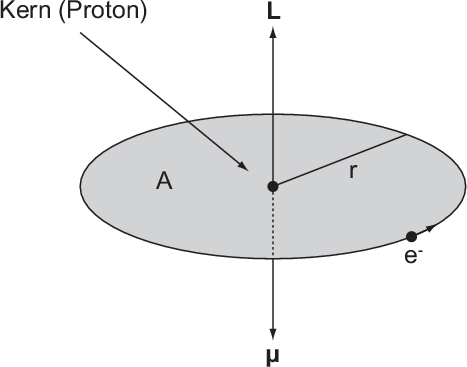
\includegraphics[width=\linewidth]{images/BohrscherDrehimpuls.png}
  \caption{\cite{ETH} Bohr'sches Modell eines Elektrons mit dem Drehimpuls $\vec{L}$ und dem magnetischen Moment $\vec{\mu}$}
  \label{fig:Bohr}
\end{figure}

Dabei ist $\vec{n}$ der Normalenvektor, senkrecht zur Kreisscheibe, auf der sich das Elektron bewegt (siehe Fig. \ref{fig:Bohr}).
Man sieht leicht, dass das magnetische Moment dem Drehimpuls des Elektrons ähnelt.
\begin{equation} \label{eq:2}
\vec{l} = \vec{r} \times \vec{p} = m_e r v \cdot \vec{n}
\end{equation}

Legt man nun ein externes Magnetfeld $\vec{B}$ an, so wechselwirkt dieses mit dem magnetischen Moment des Elektrons, sodass es zu einer Änderung des Energieniveaus kommt.
\begin{equation} \label{eq:3}
\Delta E_{Pot} = -\vec{\mu}_l \cdot \vec{B} = \frac{e}{2m_e} \cdot \vec{l} \cdot \vec{B}
\end{equation}
Nun quantisiert man den Drehimpuls des Elektrons entlang des magnetischen Feldvektors $\vec{B}$
\begin{equation} \label{eq:4}
|\vec{l}| = \sqrt{l(l+1)}\hbar \qquad l = 0, 1,…, n-1
\end{equation}
\begin{equation} \label{eq:5}
l_z = m_l \hbar \qquad -l \leq m_l \leq l
\end{equation}

Damit lässt dich die Energiedifferenz $\Delta E_{Pot}$ vereinfachen zu

\begin{equation} \label{eq:6}
\Delta E_{Pot} = \frac{e \hbar}{2 m_e} m_l B = \mu_B \cdot m_l \cdot B
\end{equation}

Hier beschreibt $\mu_B$ das von uns gesuchte Bohr'sche Magneton.
Die Änderung des Energieniveaus um $\Delta E_{Pot}$ bewirkt die Aufspaltung des ursprünglichen Energieniveaus mit Drehimpuls $l$ in $2l+1$ Unterniveaus mit demselben Drehimpuls $l$ aber unterschiedlichem $m_l$.

Alternativ kann man diese Gleichung auch quantenmechanisch herleiten. Dafür betrachtet man alle Spins und Drehmomente der Elektronen eines Atoms als einzelne Summen, sowie den Gesamtspin $\vec{J}$, die für den Hamilton-Operator im externen Magnetfeld benötigt werden. Damit erhält man die Gleichung
\begin{equation} \label{eq:7}
\Delta E_{Pot} = \mu_B \cdot M_J \cdot B \cdot g_j
\end{equation}
 Mit $g_j$ dem Landé-Faktor, der aber für den normalen Zeeman-Effekt 1 ist, wodurch (\ref{eq:7}) gleich zu (\ref{eq:6}) wird. In unserem Fall interessiert nur der normale Zeeman-Effekt.
 
 \begin{figure}
  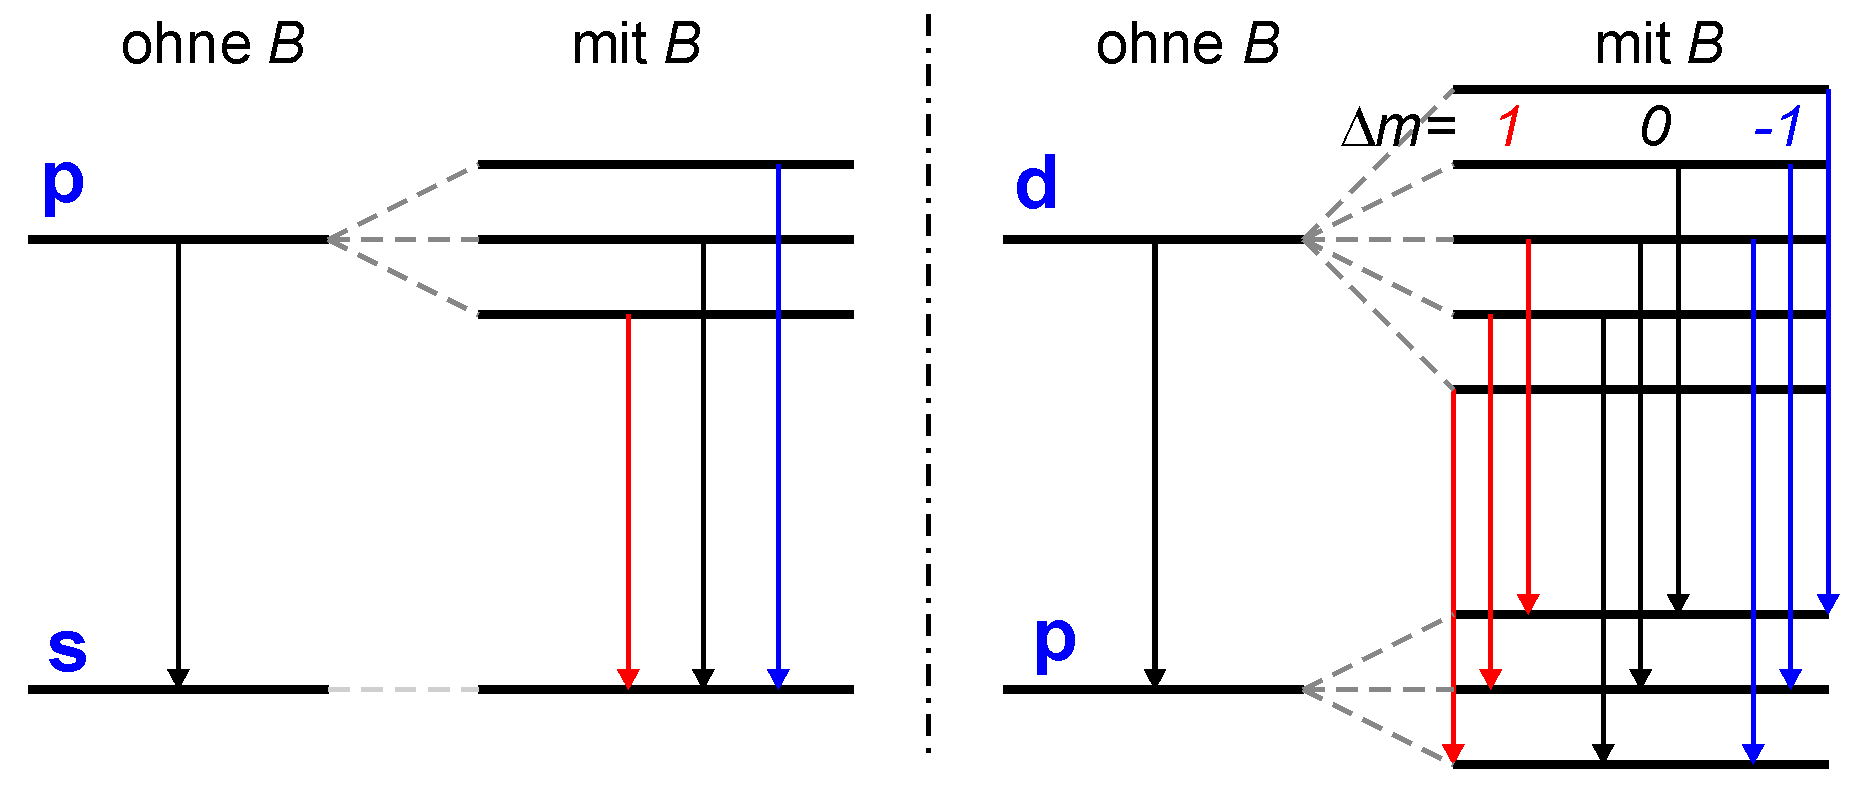
\includegraphics[width=\linewidth]{images/ZeemanAufspaltung.png}
  \caption{\cite{UniStuttgart} Aufspaltung der Energieniveaus für den normalen (links) und anormalen (recht) Zeeman-Effekt}
  \label{fig:Energieniveaus}
\end{figure}


\subsection{Auswahlregeln und Polarisation des Lichts}
Wenn ein Elektron zwischen zwei Elektronenschalen ($E_1, E_2$) "springt", so emittiert es ein Photon mit einer Wellenlänge $\lambda$, die von der Energiedifferenz der Elektronenschalen abhängt.
\begin{equation} \label{eq:8}
\frac{hc}{\lambda} = E_{ph} = \Delta E = E_1 - E_2
\end{equation}

Jedoch gibt es Einschränkungen, welche Übergänge möglich sind. Wichtig hierfür ist das Dipol-Matrixelement $M_{ik}$
\begin{equation} \label{eq:9}
M_{ik} = e \int \psi_i^* \vec{r} \psi_k dV
\end{equation}
$M_{ik}$ beschreibt die Übergangswahrscheinlichkeit zwischen den Elektronenschalen $k$ nach $i$ und muss mindestens eine Komponente besitzen, die nicht-Null ist, damit ein Übergang von  $k$ nach $i$ möglich ist.
Schreibt man (\ref{eq:9}) in alle drei Raumrichtungen um entstehen drei Integrale. So bekommt man die folgenden Vorschriften für die magnetische Quantenzahl $M$, den Drehimpuls $L$ und den Spin $S$
\begin{equation} \label{eq:10}
\Delta M_J = M_{J,i} - M_{J,k} = 0, \pm 1
\end{equation}
\begin{equation} \label{eq:10}
\Delta L = L_i - L_k = \pm 1
\end{equation}
\begin{equation} \label{eq:10}
\Delta S = 0
\end{equation}

Angenommen, der magnetische Feldvektor $\vec{B}$ zeigt in die z-Richtung, so kann nur das Matrixelement $(M_{ik})_z$ nicht-Null werden für $\Delta M_J = 0$. Diese Übergange nennt man $\pi$-Übergänge. Diese sind äquivalent dazu, dass ein Dipol entlang der z-Achse oszilliert, wodurch entlang der z-Richtung keine Strahlung emittiert wird. In die beiden anderen Richtung ist diese Oszillation des Dipols als linear polarisiertes Licht zu beobachten.
Ist dagegen $\Delta M_J = \pm 1$, so erhalten wir $\sigma$-Übergänge, für die die z-Komponente der Dipol-Matrix null wird und die x- und y-Komponenten ungleich null, jedoch zueinander um $\pi$/2 phasenverschoben. Dies führt dazu, dass wir entlang der z-Achse zirkular polarisiertes Licht beobachten und entlang der x- und y-Achse linear polarisiertes Licht.
\begin{figure}
  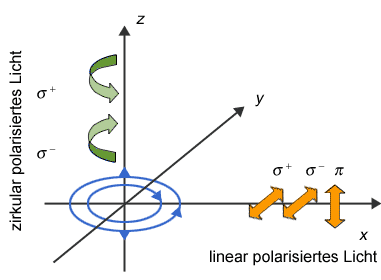
\includegraphics[width=\linewidth]{images/Polarisation.png}
  \caption{\cite{Chemga} Darstellung der Polarisation anhand der x- und z-Richtung}
  \label{fig:Polarisation}
\end{figure}

Die Beobachtungsrichtung entlang der z-Achse wird longitudinal genannt und es sollten für $\Delta M_J = + 1$ und $\Delta M_J = - 1$ je eine zirkular polarisierte $\sigma$-Linie zu sehen sein. Im Gegensatz dazu sollten in transversaler Richtung (senkrecht zur z-Achse) eine linear polarisierte $\pi$-Linie für $\Delta M_J = 0$ und zwei ebenfalls linear polarisierte $\sigma$-Linien zu beobachten sein.


\section{Durchführung und Auswertung}

\subsection{Versuchsteil 1: Spektroskopie des Zeeman-Effekts}
Im ersten Versuchsteil wurde der Zeeman-Effekt anhand der roten Cadmium-Linie untersucht, welche beim Übergang von $^1D_2 \rightarrow ~^1P_1$ entsteht.

Dazu sollte zunächst untersucht werden, ob bei den verwendeten Magneten ein Hysterese-Effekt auftritt. Dafür wurde je drei Mal eine Messung mit einer Hall-Sonde bei zu- und abnehmender Feldstärke im relevanten Bereich durchgeführt und die Ergebnisse für $B_{inc}$ und $B_{dec}$ gemittelt. In Fig. \ref{fig:Hysterese} sieht man die Ergebnisse dieser Messung. Man erkennt, dass es einen kleinen Unterschied zwischen den Messungen gibt, jedoch offenbart der Fit, dass dieser Unterschied innerhalb des Fehlers liegt, weshalb man in unserem Fall von keinem signifikanten Effekt reden kann.
\begin{figure}
  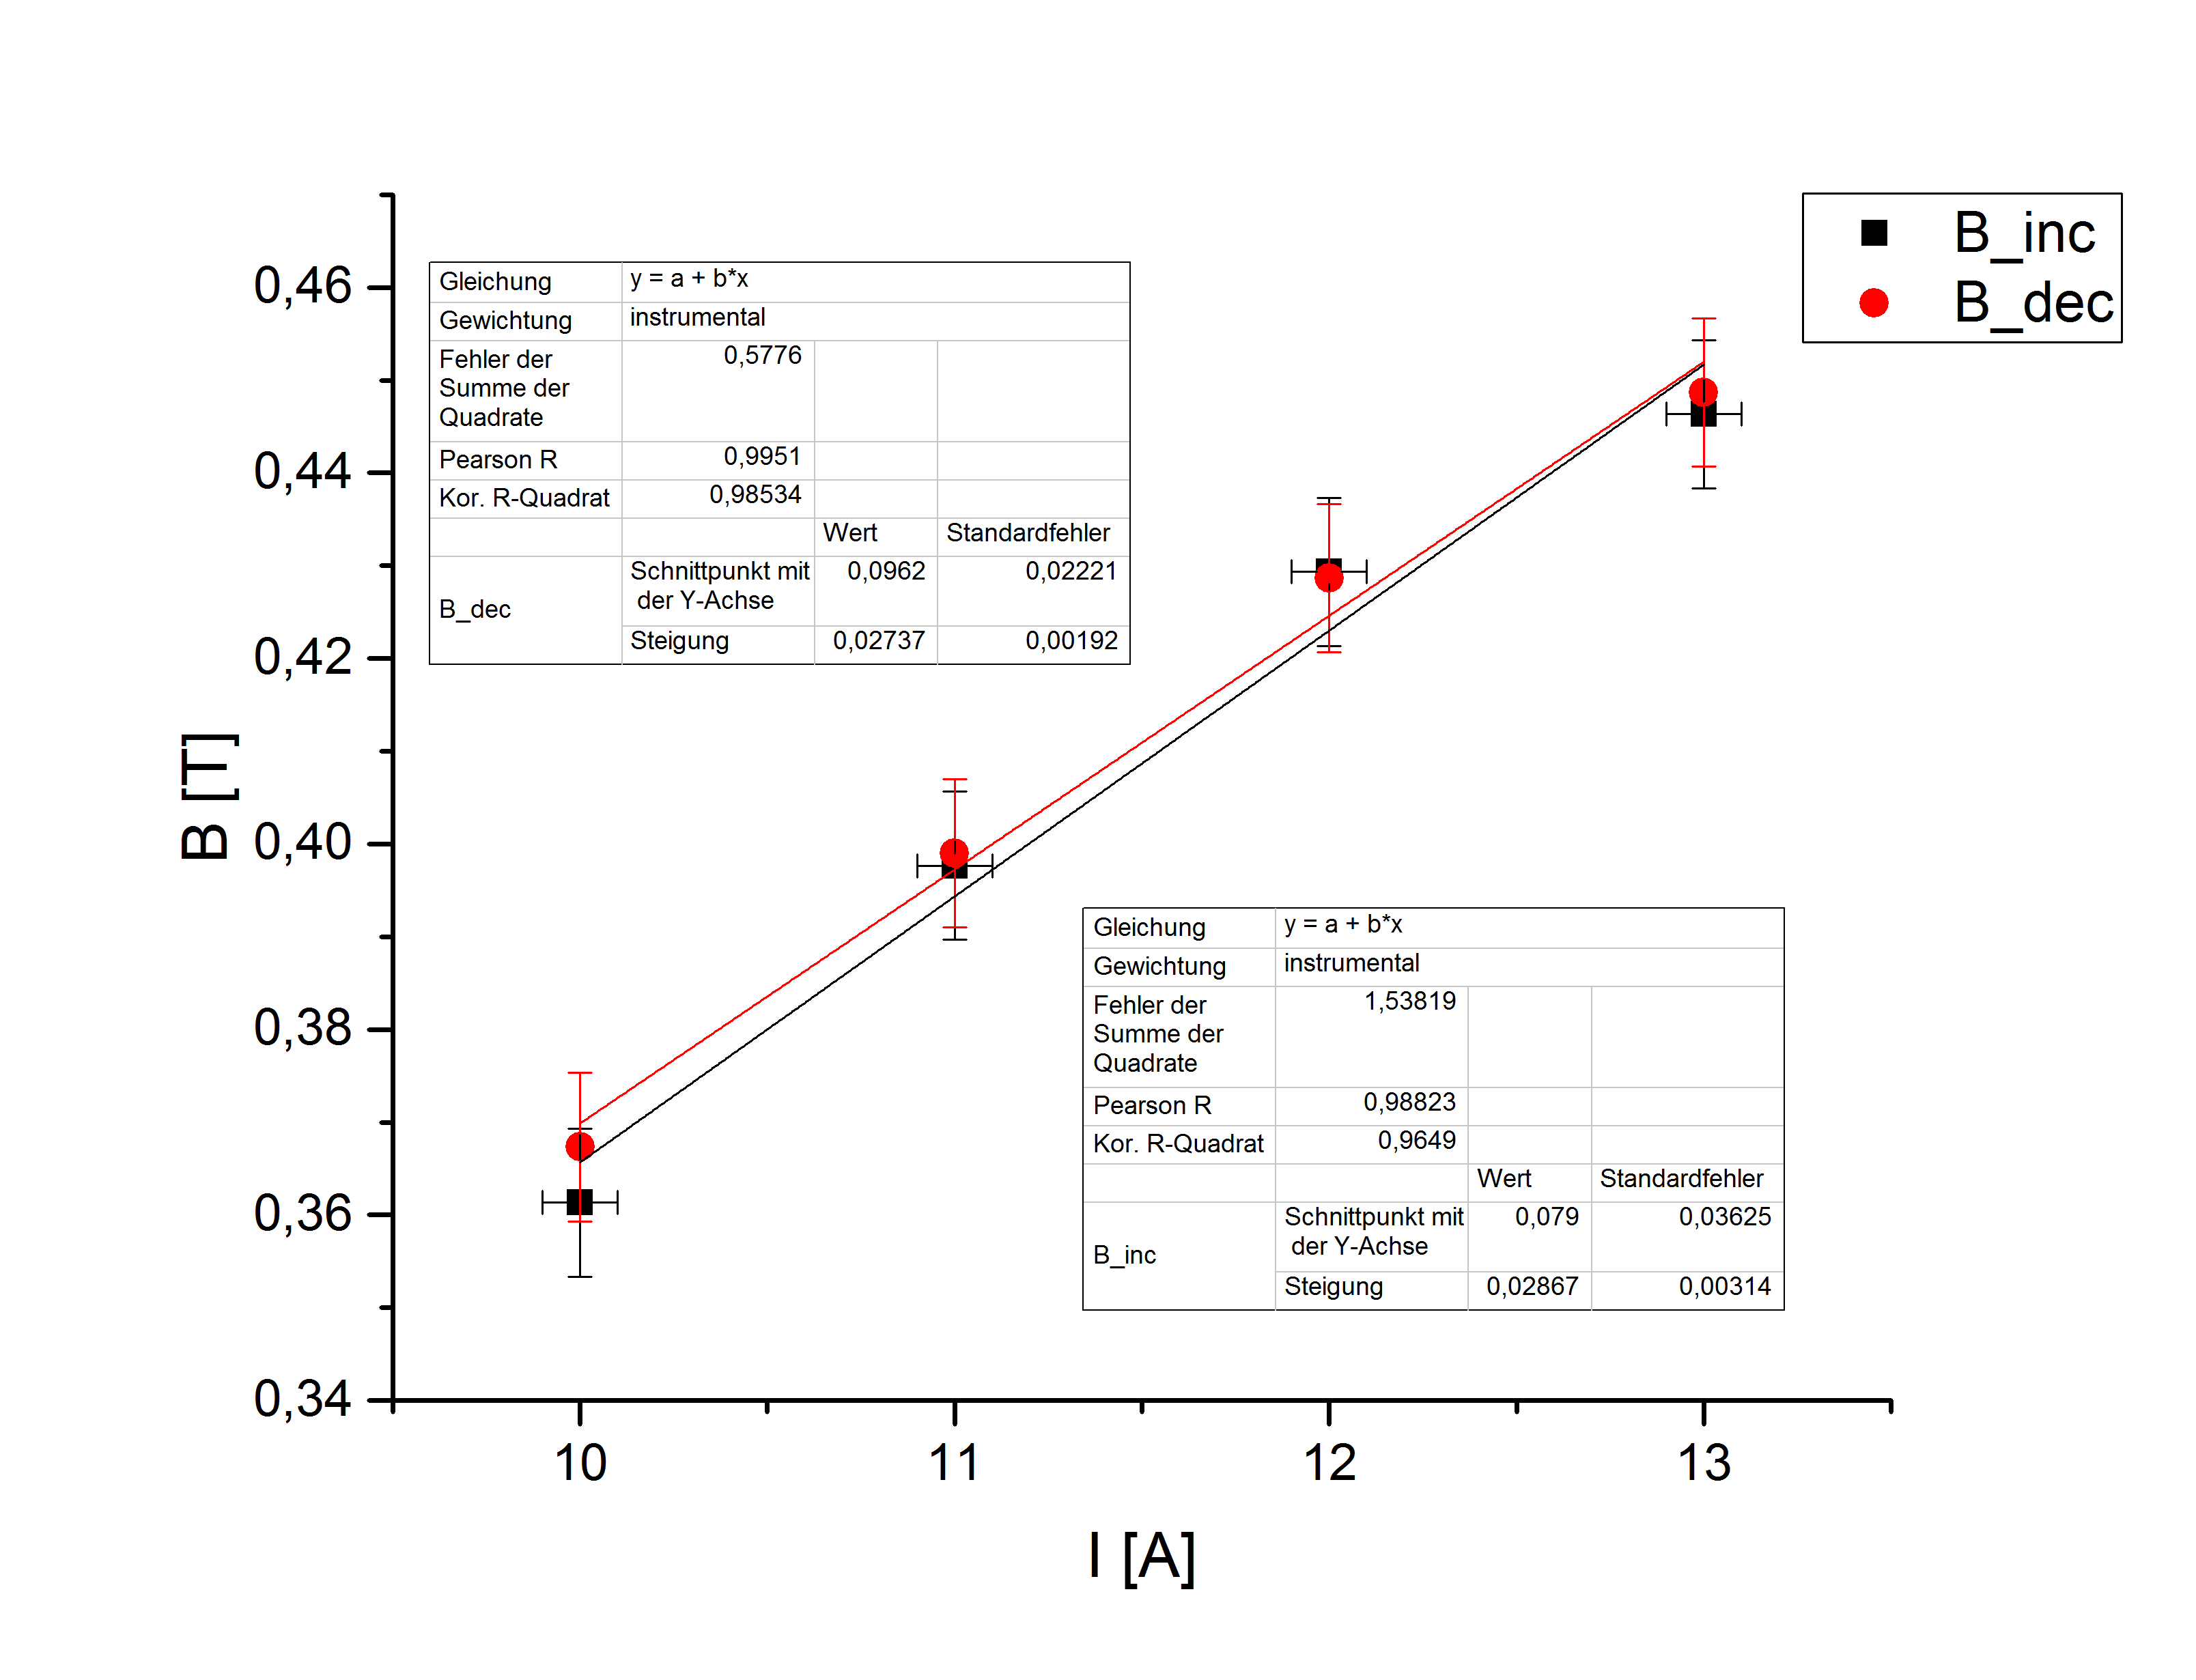
\includegraphics[width=\linewidth]{images/Hysterese.png}
  \caption{Vergleich der magnetischen Feldstärke bei zu- und abnehmender Stromstärke}
  \label{fig:Hysterese}
\end{figure}

Als nächstes sollte der Zeeman-Effekt in longitudinaler und transversaler Richtung qualitativ untersucht werden. Dazu verwendeten wir den in Fig. \ref{fig:Aufbau} dargestellten Aufbau.
\begin{figure}
  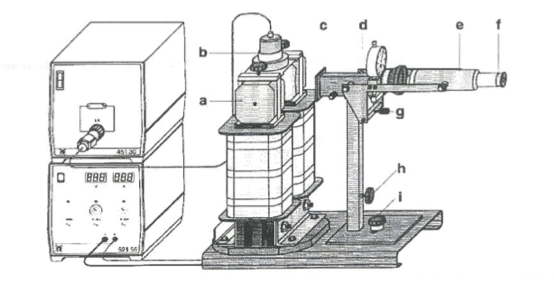
\includegraphics[width=\linewidth]{images/Aufbau.png}
  \caption{\cite{Skript} Versuchsaufbau nach dem Skript: (Darstellung aus Leybold, Physics Leaflets). a) Polschuhe des Magneten, b) Cd-Lampe, c) Rotlicht Filter, d) Lummer-Gehrcke Platte, e) Teleskop, f) Okular, g) Höheneinstellung für das Teleskop, h) Feststellschraube für die Teleskophalterung, i) Feststellschraube für die Grundplatte.}
  \label{fig:Aufbau}
\end{figure}

Das wichtigste Element dieses Aufbaus ist die Lummer-Gehrcke-Platte. Dabei handelt es um eine dünne Glasplatte mit nahezu plan-parallelen Flächen. Tritt Licht durch ein Prisma mit dem Einfallswinkel $\beta$ in die Platte ein, so wird dieses innerhalb der Platte reflektiert. Nach jeder Reflexion wird etwas Licht an der Oberfläche gebrochen, das mit Hilfe einer Linse fokussiert und zur Interferenz gebracht wird. Erfüllt der Gangunterschied die Bedingung
 \begin{equation} \label{eq:11}
\Delta = 2d\sqrt{n^2-1} = k \lambda
\end{equation}
erhält man konstruktive Interferenz mit dem Gangunterschied $\Delta = \Delta_1 - \Delta_2$, dem Brechungsindex $n = n_2$, $n_1 \approx 1$, der Dicke der Platte $d$ und der Interferenzordnung $k$ (siehe Fig. \ref{fig:LG}).
\begin{figure}
  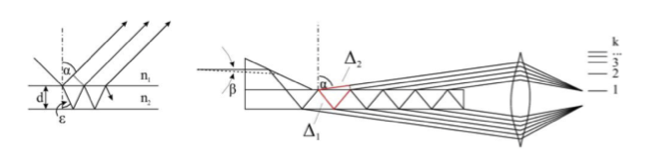
\includegraphics[width=\linewidth]{images/LGPlatte.png}
  \caption{\cite{Skript2} Funktionsweise der Lummer-Gehrcke-Platte.}
  \label{fig:LG}
\end{figure}
Der Reflexionswinkel $\alpha$ innerhalb der Platte wird als $\approx 90 \degree$ angenommen, wodurch es annähernd zu totaler Reflexion innerhalb der Platte kommt.
%eigene Idee

Das Interferenzmuster der Lummer-Gehrcke Platte für eine Aufnahme in transversaler Richtung kann in Fig. \ref{fig:Interferenz} betrachtet werden.

Mit dieser Messmethode und unter Zuhilfenahme eines Teleskops konnten wir in transversaler Richtung 3 Linien beobachten, in der Mitte die $\pi$-Linie, parallel dazu links und rechts die $\sigma_{\pm}$-Linien. Wird ein Polarisationsfilter in den Strahlengang gehalten, können wir entweder die $\pi$- oder die beiden $\sigma$-Linien komplett herausfiltern. Die drei Linien sind somit linear polarisiert, wobei die Polarisation der $\pi$-Linie senkrecht zu der der $\sigma_{\pm}$-Linien und parallel zu den B-Feldlinien ist.
In longitudinaler Richtung können wir die $\sigma_+$- und $\sigma_-$-Linie beobachten. Es ist nicht möglich, allein mit dem Polarisationsfilter eine Linie auszublenden, hält man jedoch noch ein $\lambda/4$-Plättchen vor den Polarisationsfilter, das aus zirkular polarisiertem Licht linear polarisiertes Licht macht, so kann man mit dem Polarisationsfilter je eine der beiden Linien unter Drehung um 90$\degree$ ausblenden. Dies lässt auf rechts- bzw. links-polarisiertes Licht schließen.

\begin{figure}
  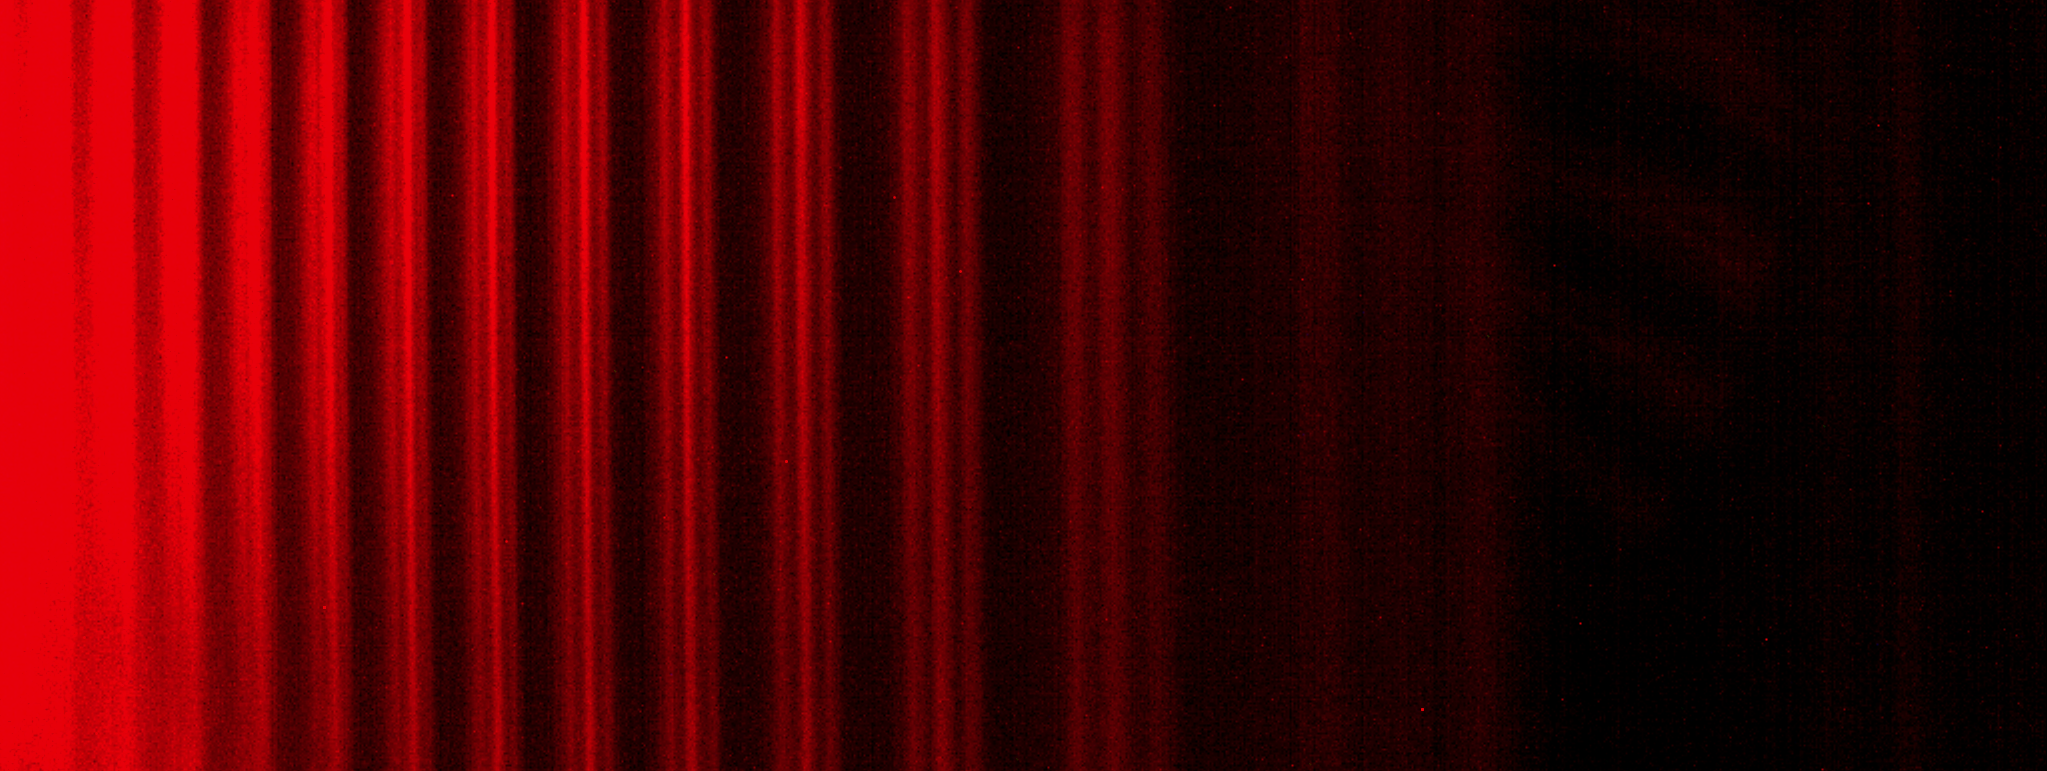
\includegraphics[width=\linewidth]{images/Transversal.png}
  \caption{Zeeman-Effekt in transversaler Richtung bei $I = 13 A$.}
  \label{fig:Interferenz}
\end{figure}

\begin{figure}
  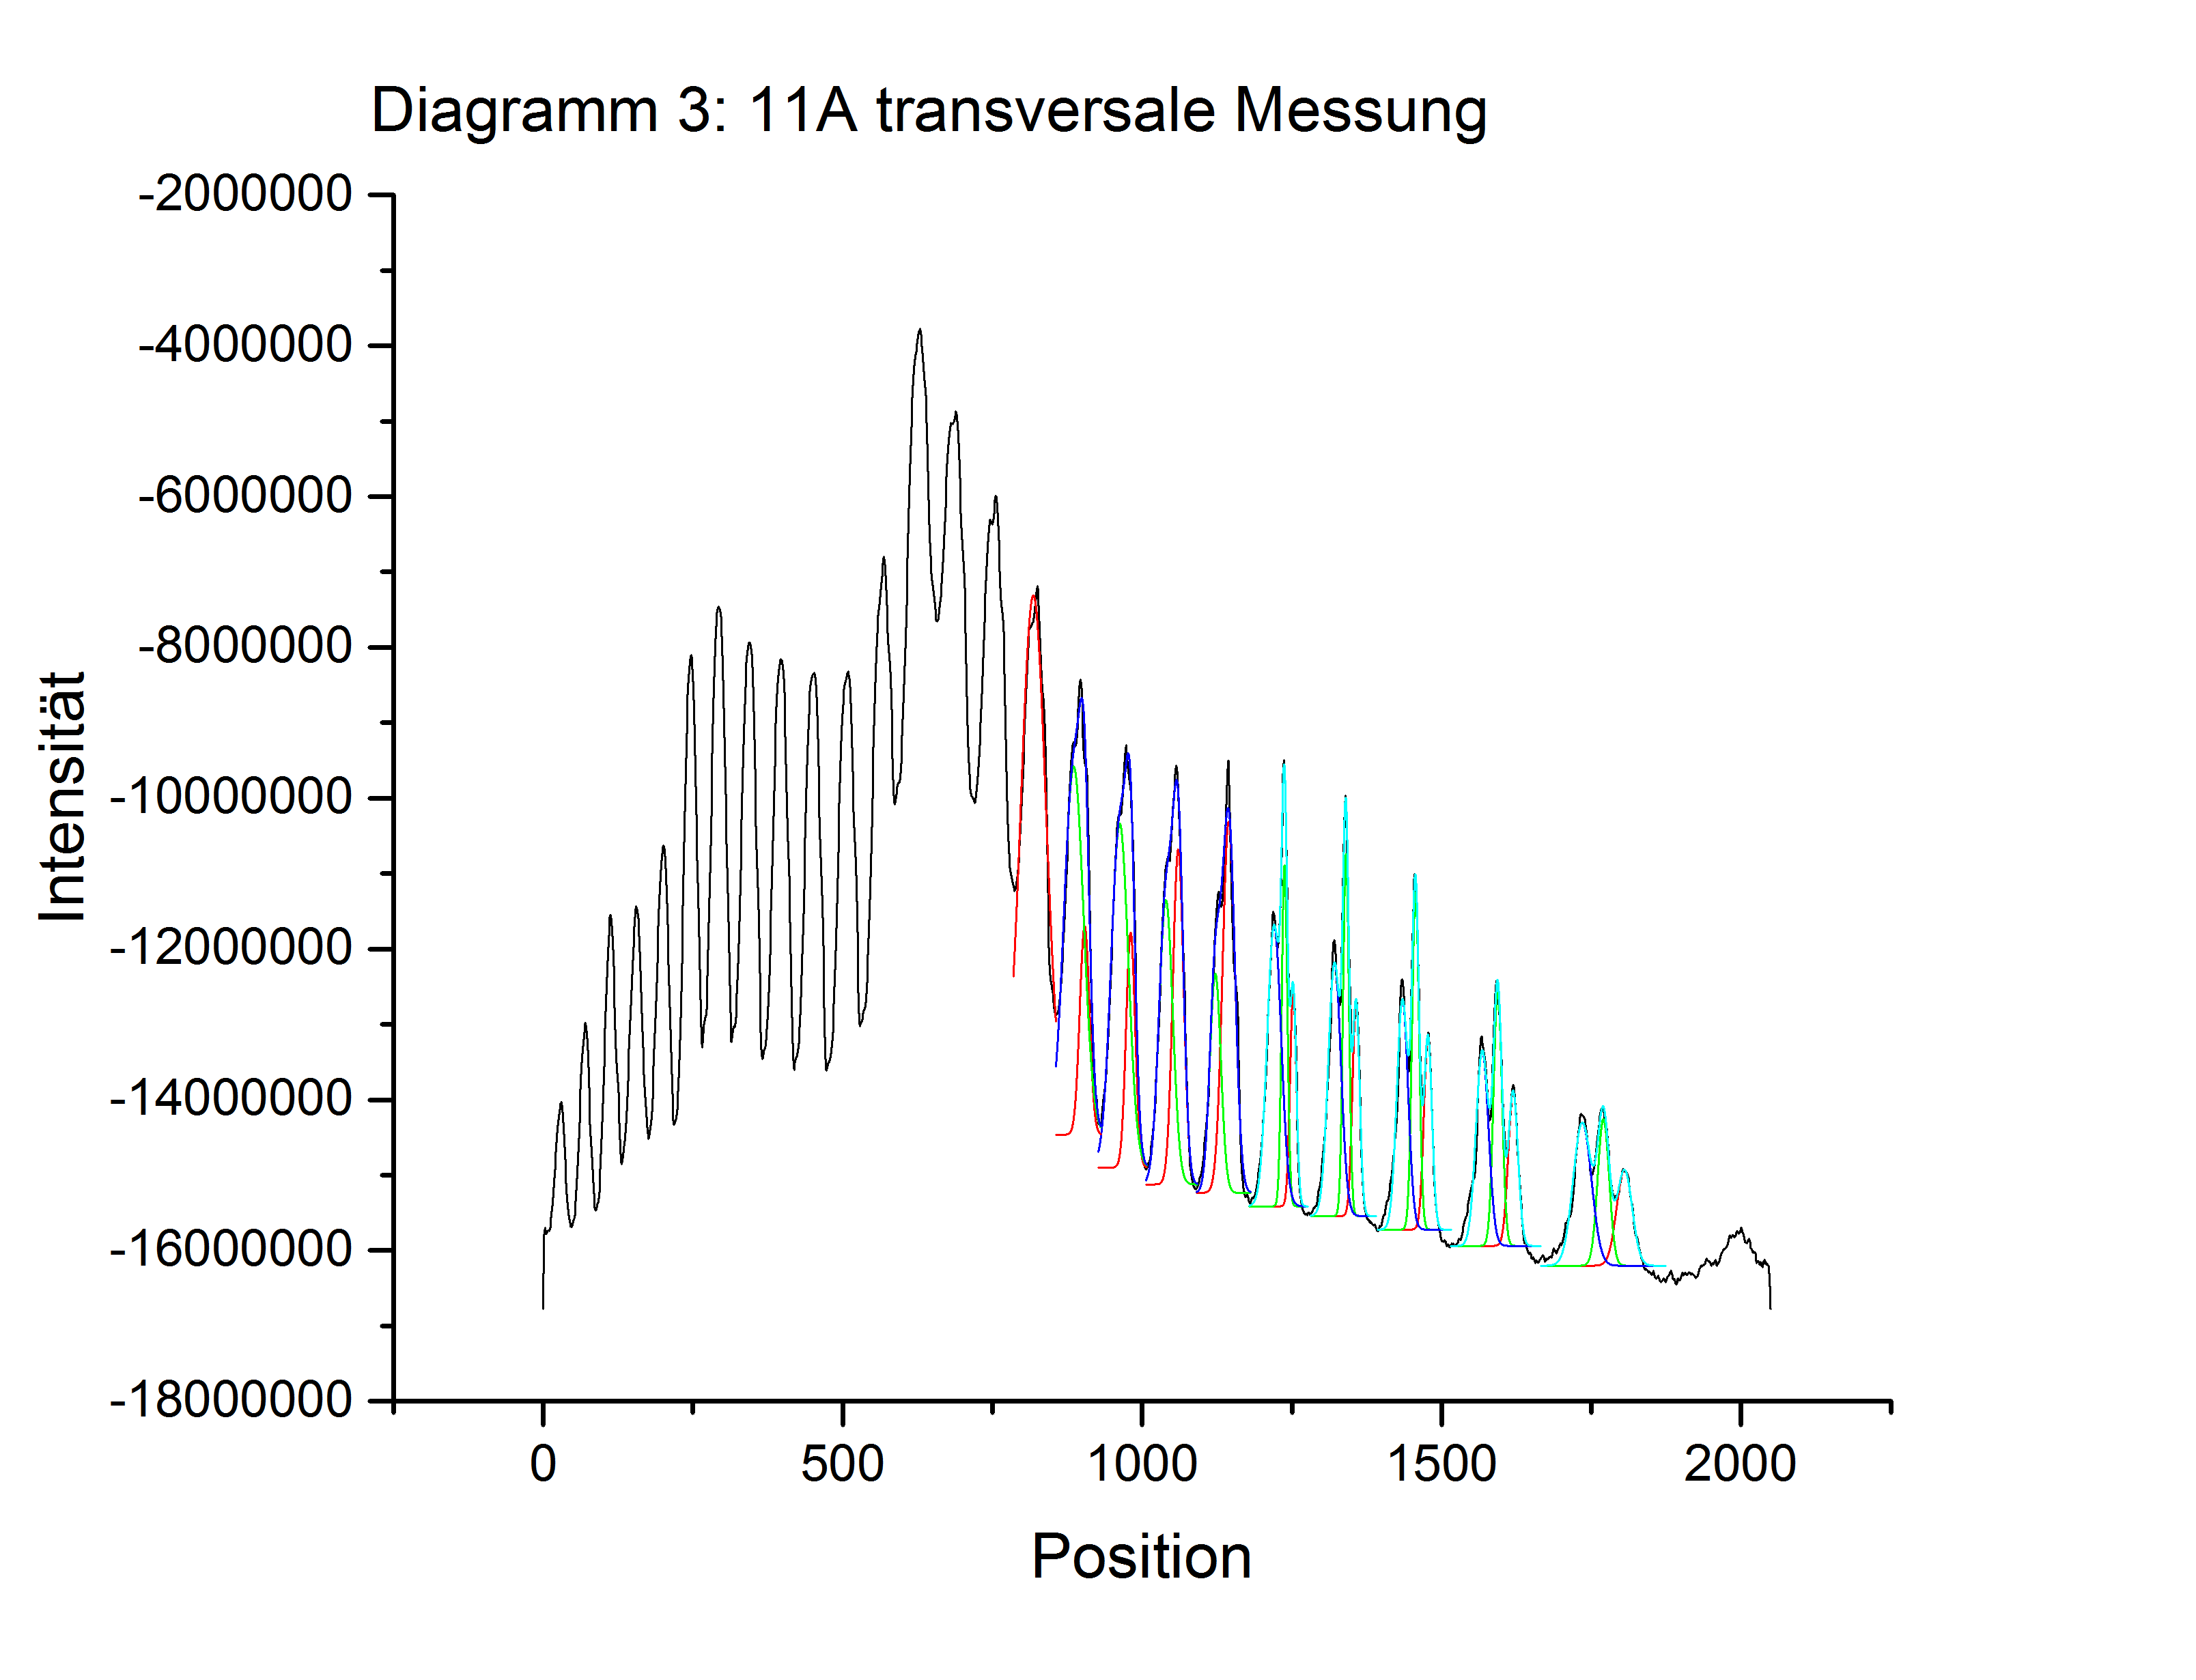
\includegraphics[width=\linewidth]{images/11AMessung.png}
  \caption{Zeeman-Effekt in transversaler Richtung bei $I = 11 A$ entlang der y-Achse integriert. Nicht aus derselben Messreihe wie Fig. \ref{fig:Interferenz}!}
  \label{fig:Gaussfits}
\end{figure}

Die quantitativen Ergebnisse aus der Beobachtung der Zeeman-Effekts sollten als nächstes dazu verwendet werden, das Bohr'sche Magneton zu bestimmen. Dazu wurden die Aufnahmen aus dem ersten Versuchsteil mit dem Programm ImageJ entlang der Y-Achse integriert und mit "multiple peaks" in Origin Gauß-gefittet. Dadurch erhielten wir die Positionen und die Breite der Interferenzlinien in Pixel für jede Messung mit $I = 10, 12$ und $13 A$. Die Ordnungen der $\pi$-Linie wurden dann gegen die Position in Pixel geplottet und mit einem polynomialen Fit zweiter Ordnung versehen. Mit Hilfe dieses Fits wurden die Ordnungen der $\sigma$-Linien bestimmt.

Um daraus das Bohr'sche Magneton bestimmen zu können, benutzen wir folgenden Ansatz:

Betrachtet man den Abstand zwischen den $\pi$- und $\sigma$-Linien, so kann man die Wellenlängen als $\lambda$ und $\lambda + \delta \lambda$ identifizieren. Dabei gilt für $\delta \lambda$ aus der Messung
\begin{equation} \label{eq:11}
\delta \lambda = \frac{\delta k}{\Delta k} \Delta \lambda = \delta k \Delta \lambda
\end{equation}
mit $\Delta k$ der Ordnungsdifferenz zwischen zwei $\pi$-Linien, $\delta k$ der Ordnungsdifferenz zwischen $\pi$- und $\sigma$-Linie und $\Delta\lambda$ bestimmt durch
\begin{equation} \label{eq:12}
\Delta \lambda = \frac{\lambda^2}{2d \sqrt{n^2 -1}} 
\end{equation}

Damit ergibt sich für $\delta \lambda$ in Abhängigkeit von $\delta k$
\begin{equation} \label{eq:13}
\delta \lambda = \delta k \frac{\lambda^2}{2d \sqrt{n^2 -1}}
\end{equation}
mit $n = 1,457$ und $d = 4,04 mm$. Für diese Messung ist $\lambda$ die Wellenlänge der roten Cadmium-Linie, welche wir im zweiten Versuchsteil (siehe (\ref{res:b})) als $\lambda_{Cd} = (643,84 \pm 0,05) nm$ bestimmt haben.

Verwendet man die Energiedifferenz $\Delta E_{pot}$ zweier Wellenlängen
\begin{equation} \label{eq:14}
\Delta E_{pot} = hc (\frac{1}{\lambda_1}-\frac{1}{\lambda_2}) \approx hc \frac{\delta \lambda}{\lambda_1^2}
\end{equation}
und setzt diese mit der Energiedifferenz der zugehörigen Energieniveaus aus (\ref{eq:6}) gleich, so erhält man
\begin{equation} \label{eq:15}
\mu_B = \frac{hc}{2Bd \sqrt{n^2 -1}} \delta k
\end{equation}

In unserem Versuch ergab sich ein mittleres Bohr'sches Magneton von
\[
\mu_B = (9,5 \pm 1,4) \times 10^{-24} \frac{J}{T} \tag{a}
\]
Das Ergebnis für $\mu_B$ wurde aus der Messreihe in Tabelle 1 gemittelt

Der Fehler ergibt sich aus Fehlerfortpflanzung, die auf der Standardabweichung analog zur Standardabweichung der Gauß-Peaks in Fig. \ref{fig:Gaussfits} aufbaut.


\subsection{Versuchsteil 2: Präzisionssprektroskopie}

Im zweiten Teil des Versuchs sollten die Wellenlängen von zwei Linien des Cadmium-Spektrums bestimmt werden.

Hierzu wurde ein Czerny-Turner-Sprektrometer mit einer Neon-Lampe als Referenz verwendet.
Das Czerny-Turner-Spektrometer erlaubt die Wellenlängen von eintretendem Licht mit Hilfe eines Gitters spektral zu erfassen. Dazu wird das Licht, das durch eine Öffnung eintritt, durch einen konkaven Spiegel auf das Gitter fokussiert, wo es spektral aufgespaltet wird und anschließend von einem weiteren Spiegel reflektiert wird, sodass die eingebauten CCD-Kamera in der Fokusebene des Spektrums liegt.
\begin{figure}
  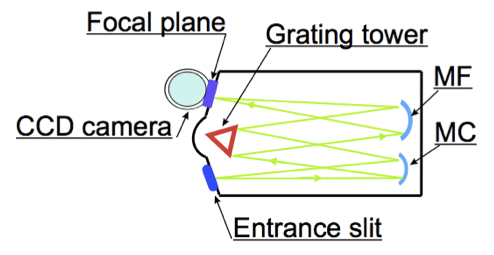
\includegraphics[width=\linewidth]{images/CTS.png}
  \caption{\cite{Skript3} Aufbau Czerny-Turner-Spektrometer.}
  \label{fig:CTS}
\end{figure}

Zunächst bestimmten wir in einer Referenz-Messung die Position der Peaks im Neon-Spektrum im Bereich um 640nm. Die Peaks in der Aufnahme des Spektrums wurden zur Bestimmung der Postion mit Gauß-Fits versehen und den passenden Wellenlängen zugeordnet.
Anschließend wurde die Wellenlänge der Peaks gegen deren Postion in Pixel aufgetragen (Fig. \ref{fig:PositionPeaks}) und mit einer polynomialen Funktion zweiter Ordnung gefittet. Als Fehler wurde die Halbwertsbreite des Fits verwendet.
\begin{figure}
  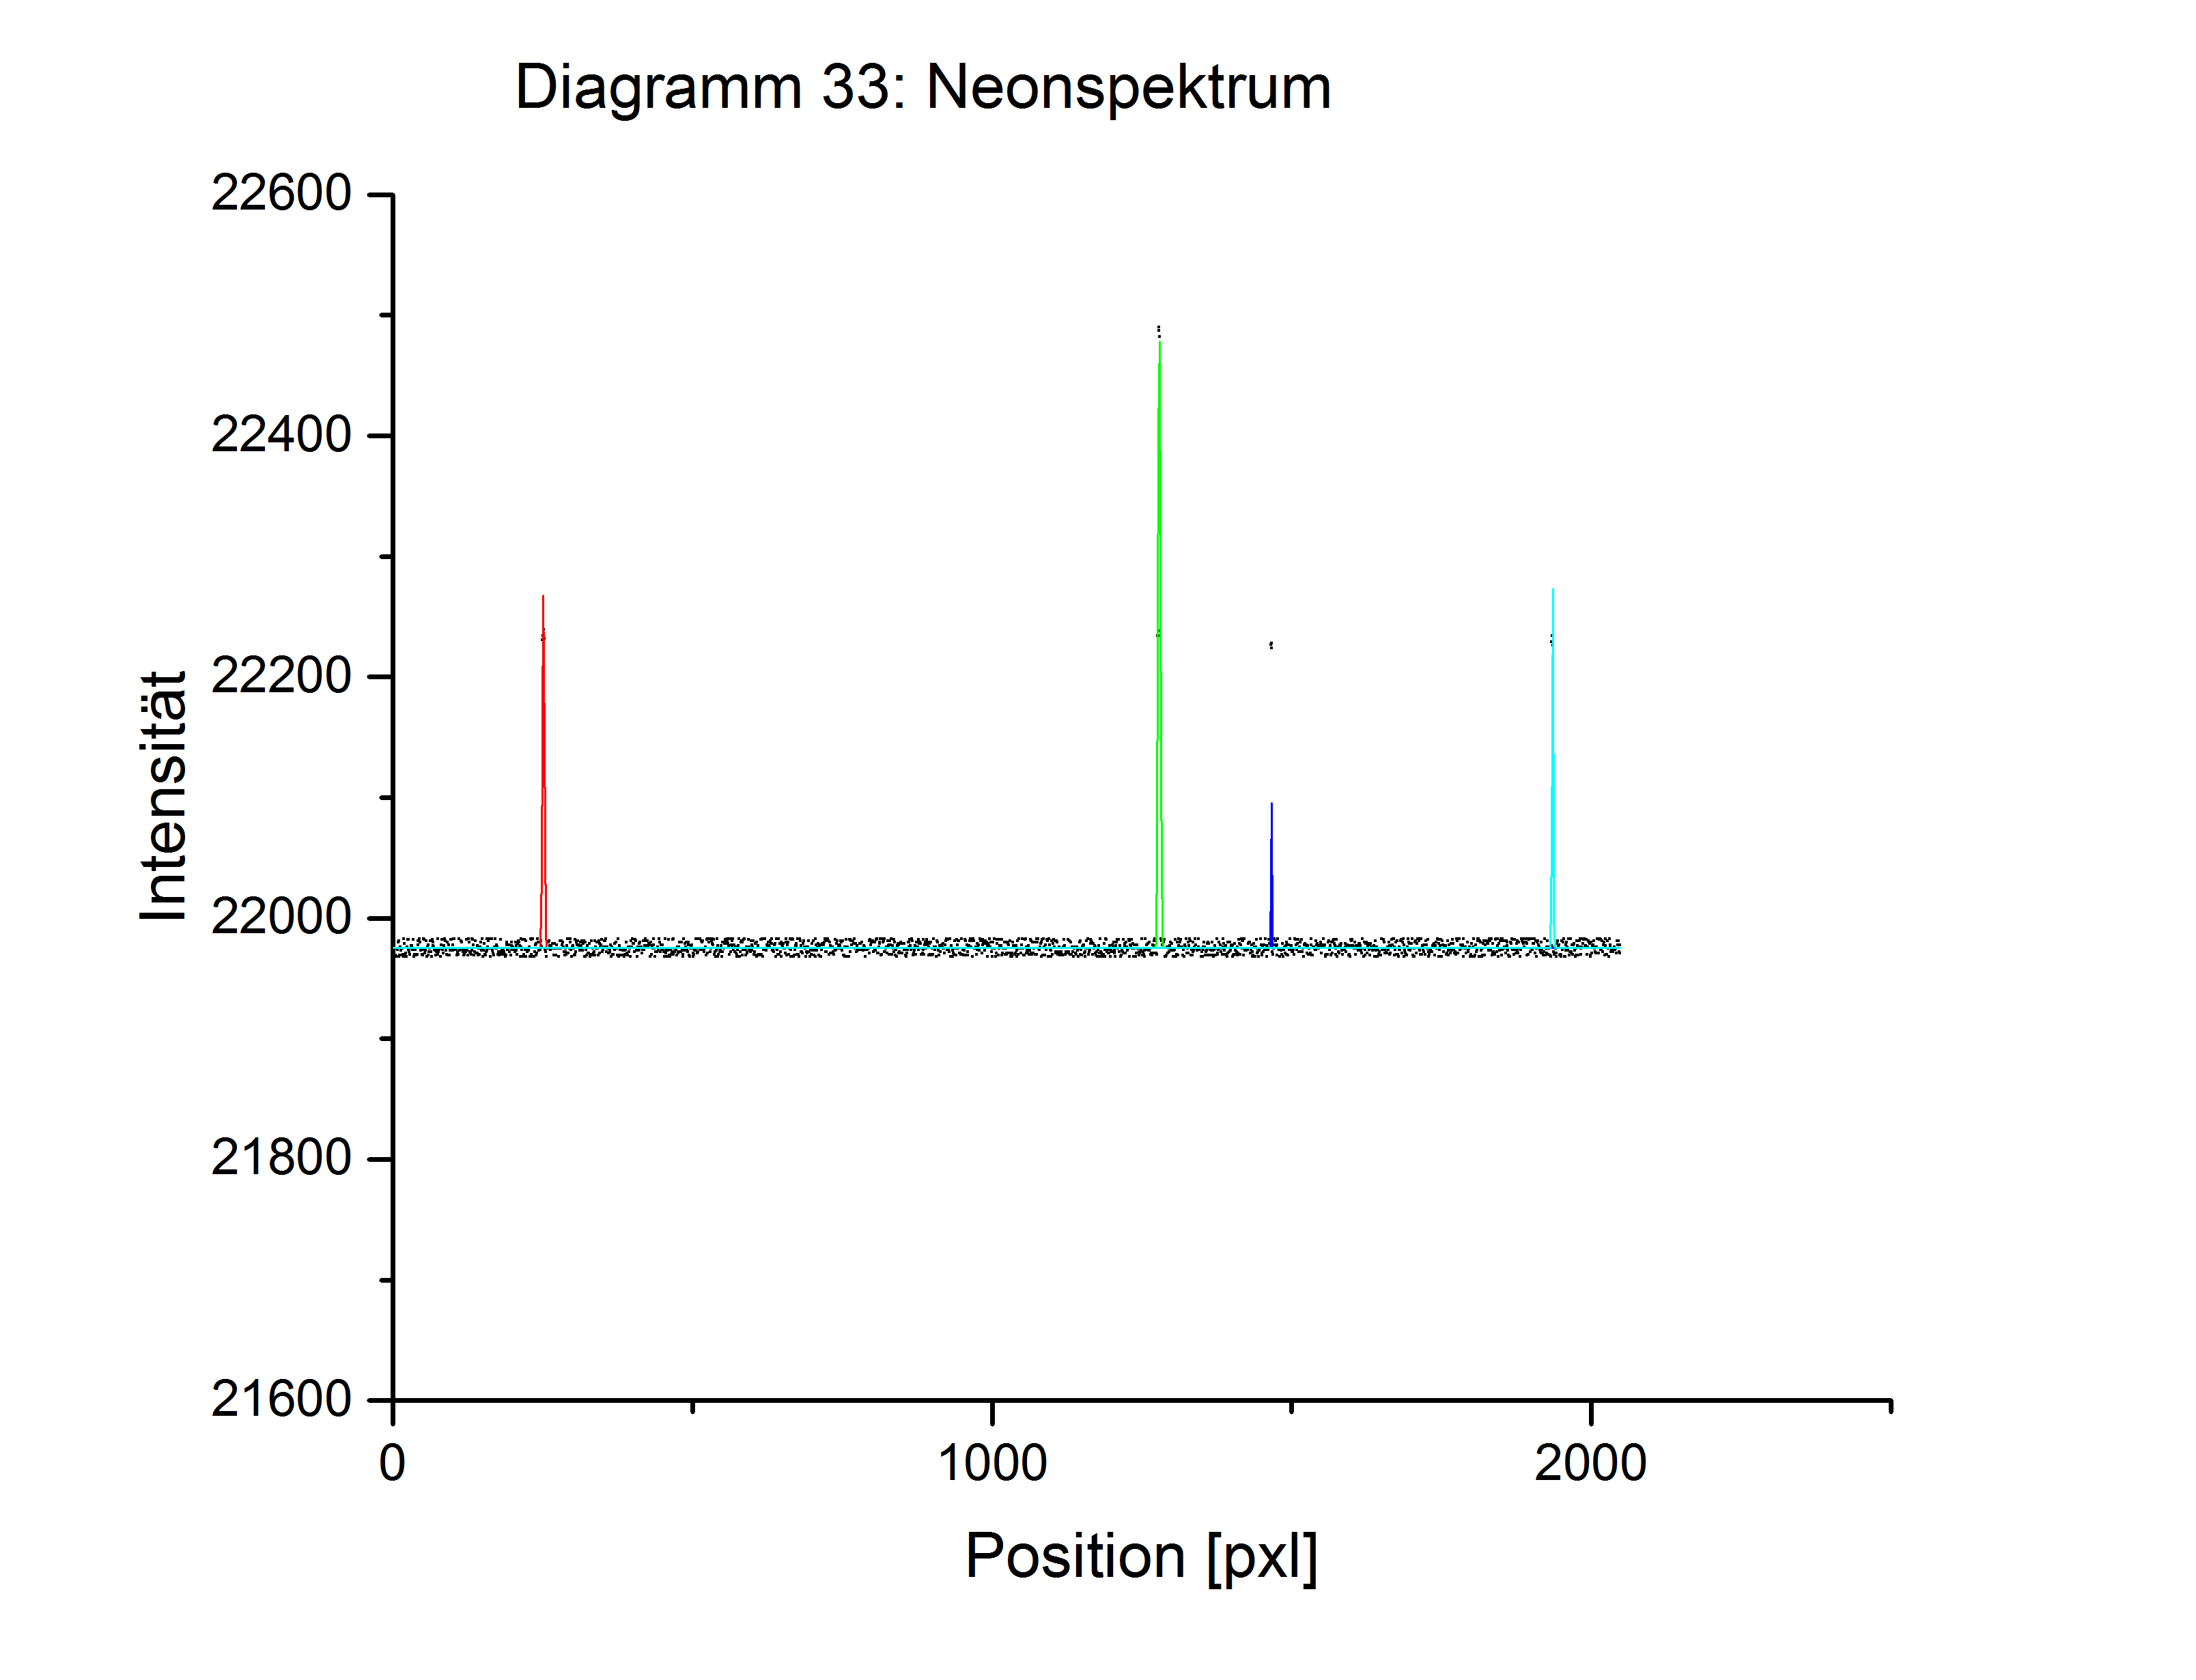
\includegraphics[width=\linewidth]{images/Neonspektrum.png}
  \caption{Aufnahme des Neon-Spektrums um $\lambda = 640 nm$}
  \label{fig:Neonspektrum}
\end{figure}

In einer zweiten Messung haben wir bei gleichen Einstellungen das Spektrum der Cadmium-Lampe aufgenommen und ebenfalls durch einen Gauß-Fit die Position der Peaks bestimmt. Aus dem Fit der ersten Messung konnten wir dann die Wellenlängen der beiden sichtbaren Linien berechnen.
\begin{figure}
  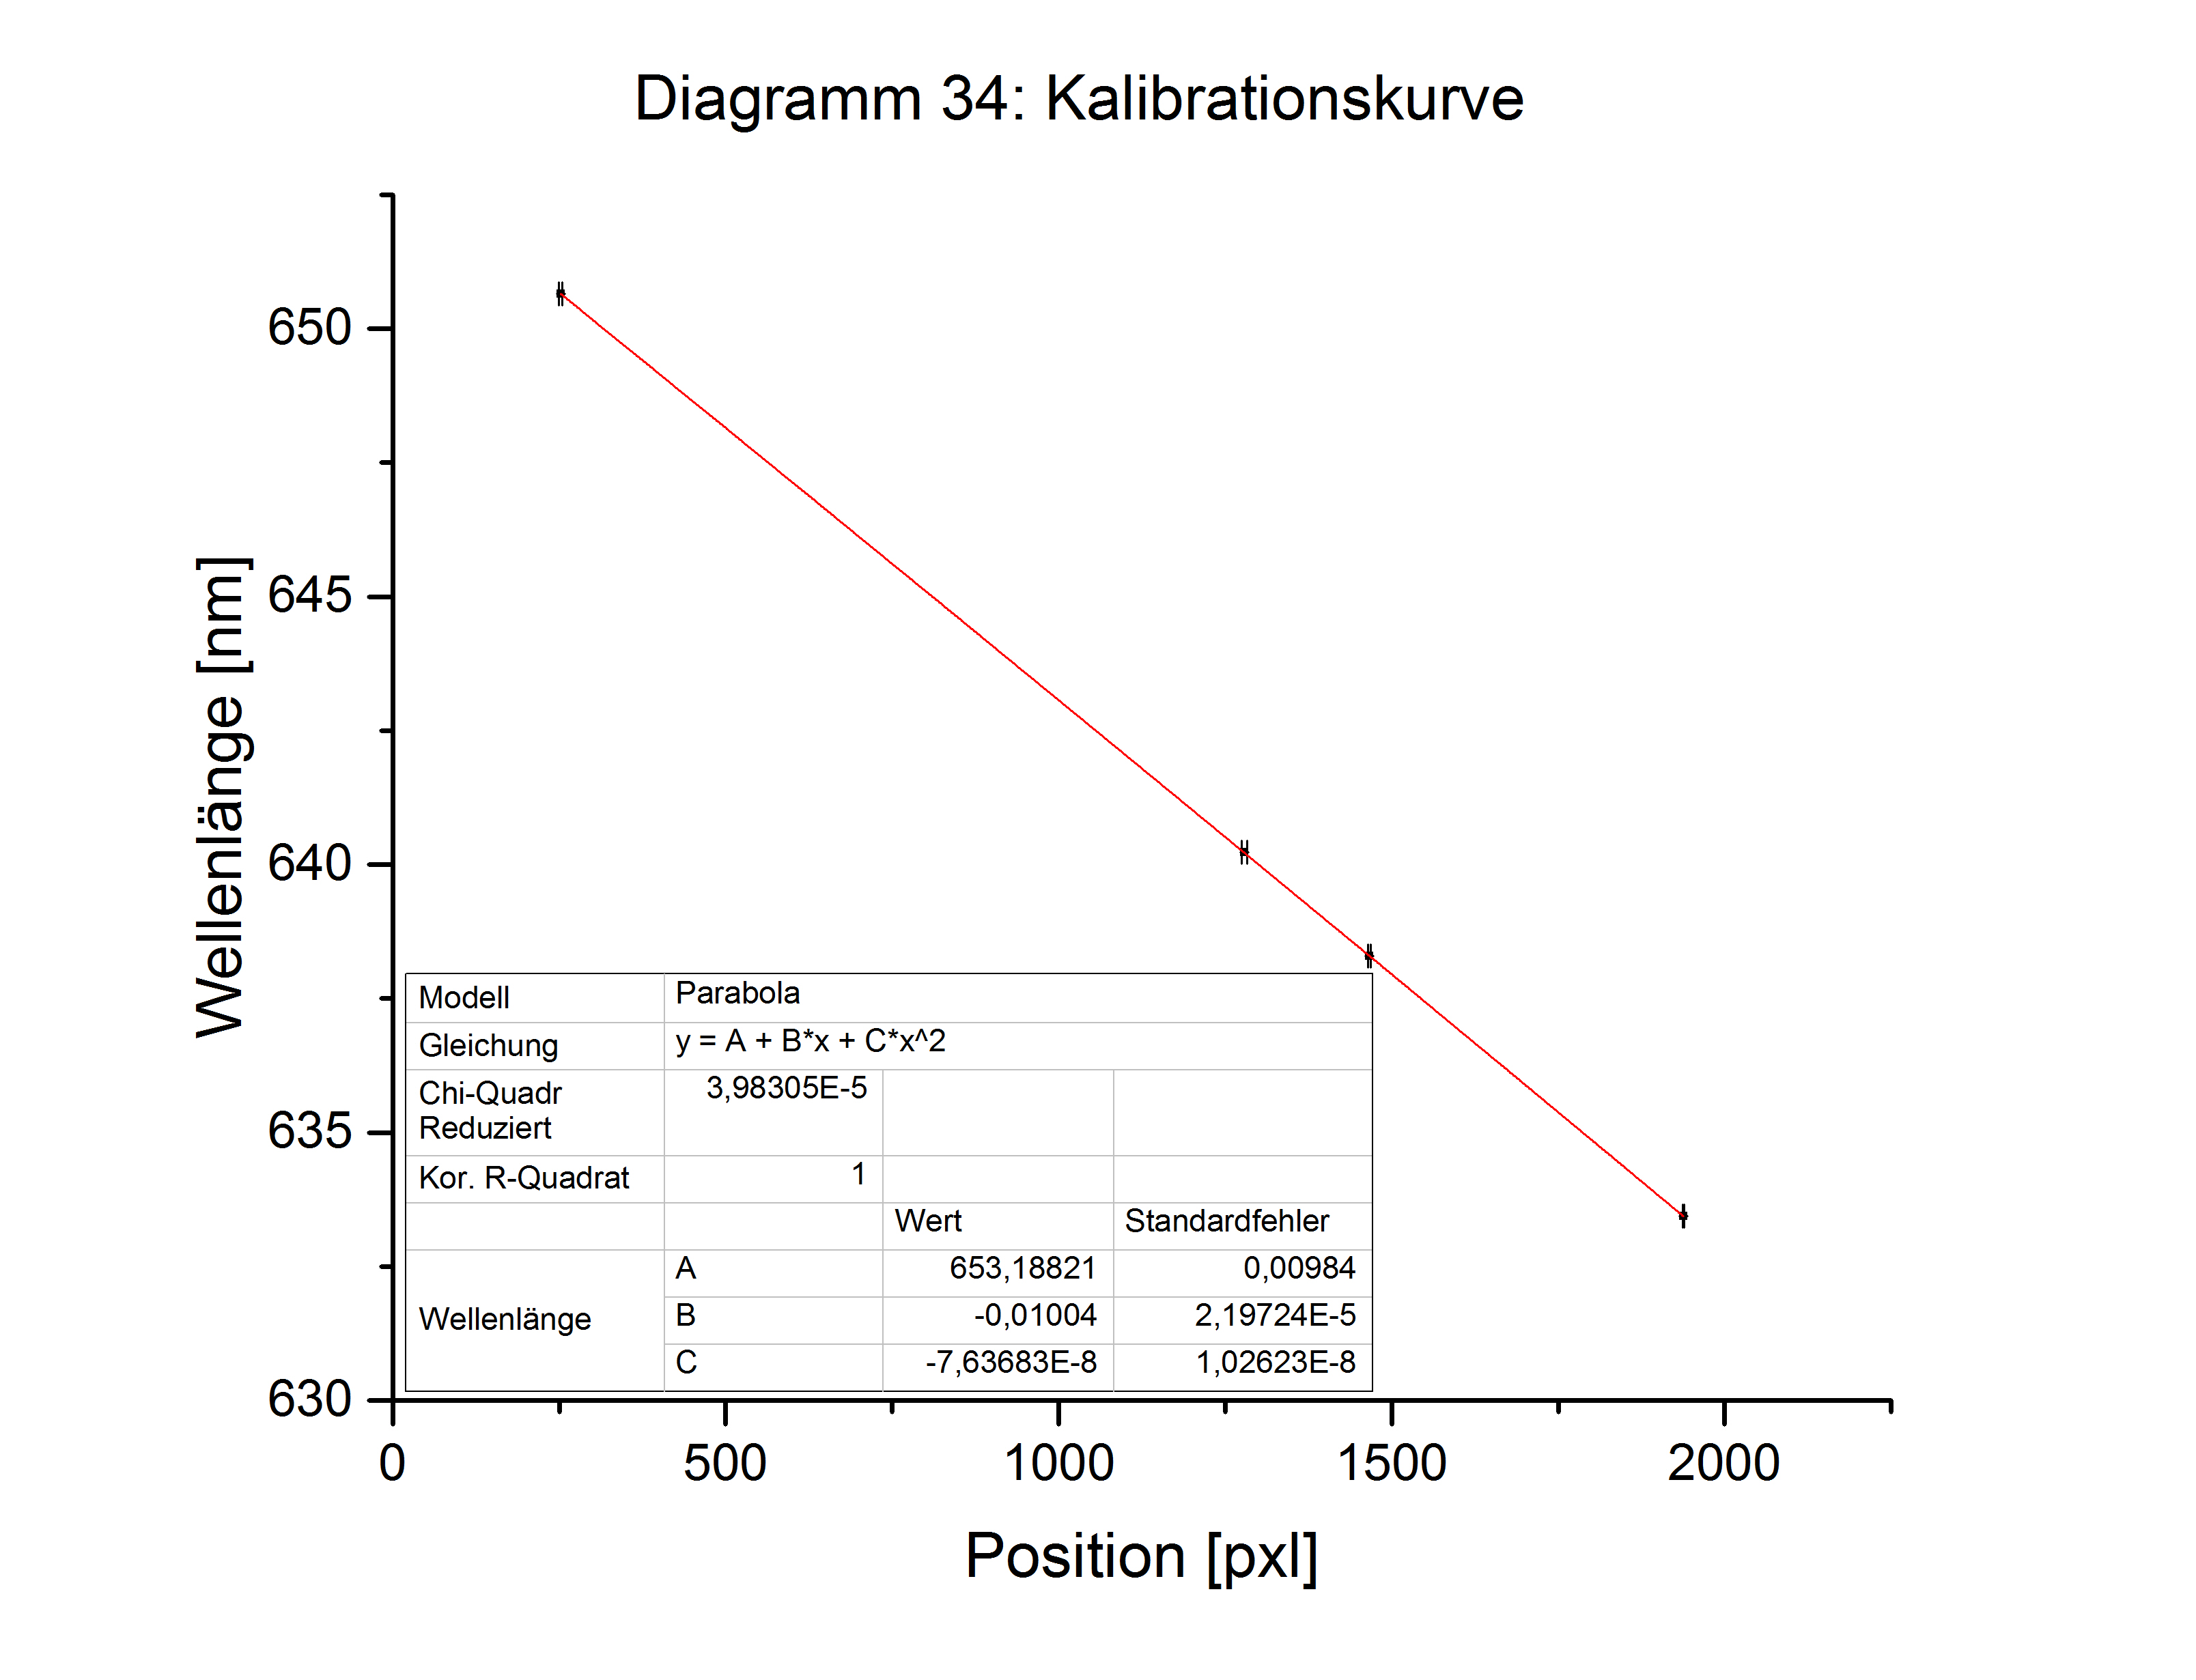
\includegraphics[width=\linewidth]{images/Kalibrationskurve.jpg}
  \caption{Position der Neon-Peaks gegen die bekannte Wellenlänge}
  \label{fig:PositionPeaks}
\end{figure}

Für die starke Cadmium-Linie erhielten wir eine Wellenlänge von
\[
\lambda_{Cd} = (643,84 \pm 0,05) nm \tag{b}\label{res:b}
\]
und für die schwache Linie eine Wellenlänge von
\[
\lambda_{unbekannt} = (652,20 \pm 0,06) nm \tag{c}
\]

Mit Hilfe der NIST Atomic Spectra Database\cite{NIST} konnten wir unser unbekanntes Element auf folgende Elemente eingrenzen:

\begin{inlineitemize}
\anitem{Schwefel} \anitem{Silizium} \anitem{Xenon} \lastitem{Wolfram}
\anitem{Thorium} \anitem{Cobalt} \lastitem{Stickstoff}
\end{inlineitemize}
Davon sind Xenon als gasförmige Verunreinigung, sowie Wolfram und Thorium als Elektrodenmaterial am wahrscheinlichsten.


\subsection{Kritische Würdigung}

Ziel des Versuches war es, anhand des Zeeman-Effekts das Bohr'sche Magneton zu bestimmen und anschließend mit Hilfe eines Czerny-Turner-Spektrometers die Wellenlängen der roten Cadmium-Linie und eines unbekannten Elements zu bestimmen.

Im ersten Versuchsteil wurde der verwendete Magnet auf Hysterese-Effekte untersucht, welche sich jedoch als vernachlässigbar herausstellten. Vermutlich überwiegten bei den dazugehörigen Messungen die äußeren Fehler, wie zum Beispiel das manuelle Einführen der Hall-Sonde.

Als nächstes wurde der Zeeman-Effekt selbst qualitativ mit einer Cadmium-Lampe beobachtet. Hierbei wurde die Polarisation, sowie die Anzahl der Interferenzlinien in longitudinaler und transversaler Richtung untersucht. Die Beobachtungen stimmten mit den vorhergehenden theoretischen Überlegungen überein.

Aus der transversalen Beobachtungsrichtung konnten wir zusätzlich noch Informationen über die Linienposition erhalten und so das Bohr'sche Magneton errechnen. Wir erhielten einen experimentellen Wert von $\mu_{B, exp} = (9,5 \pm 1,4) \times 10^{-24} \frac{J}{T}$, welcher innerhalb des Fehlerbereichs des Literaturwert $\mu_{B, lit} = 9,274 \times 10^{-24} \frac{J}{T}$ übereinstimmte. Bemerkenswert hierbei ist der große Fehler von über 14\% für den Mittelwert aus 3 Messungen. Der Fehler resultiert hauptsächlich aus der Ungenauigkeit der Fit-Kurven, da hier als Fehler der Position der Peaks die Standardabweichung verwendet wurde.

Im zweiten Teil des Versuchs sollten die Wellenlängen von Cadmium, sowie eines weiteren Elements bestimmt werden. Für die starke rote Cadmium-Linie ergab sich eine Wellenlänge von $\lambda_{Cd, exp} = (643,84 \pm 0,05) nm$, welche nicht signifikant vom Literaturwert $\lambda_{Cd, lit} = 643,847nm$ abwich.
Für das unbekannte Element, was eine Wellenlänge von $\lambda_{unbekannt} = (652,20 \pm 0,06) nm$ besaß, kamen für uns vor allem die Elemente Xenon, Wolfram und Thorium in Frage, da diese als Bauelemente oder mögliche Verunreinigungen in der Gaslampe vorkommen können.

Insgesamt verlief der Versuch somit zufriedenstellend, da alle Messwerte im Fehlerbereich mit den Literaturwerten übereinstimmten. Als mögliche Verbesserung würden wir zum einen eine optische Bank zur Befestigung der optischen Elemente vorschlagen, wodurch versehentliche Fehljustierungen seltener werden. Zum anderen wäre eine mechanische Befestigung für die Hall-Sonde von Vorteil, da der Hysterese Effekt offensichtlich sehr klein ausfällt und somit eine Fehlerquelle beseitigt werden könnte.

\appendices
\section{Wertetabellen}
\begin{minipage}{\linewidth}
\centering
\begin{tabular}{c | c | c | c | c }
  I [$A$] & B [$T$] & ${\delta k}$ & $\delta \lambda$ [$pm$] & $\mu_B$ [$10^{-24} \frac{J}{T}$] \\
  \hline
  $10,0$ & $0,37 \pm 0,05$ & $0,15 \pm 0,04$ & $7,4 \pm 1,7$ & $9,6 \pm 2,6$ \\
  $12,0$ & $0,43 \pm 0,05$ & $0,18 \pm 0,03$ & $8,5 \pm 1,6$ & $9,5 \pm 2,1$ \\
  $13,0$ & $0,46 \pm 0,06$ & $0,19 \pm 0,04$ & $9,0 \pm 2,1$ & $9,3 \pm 2,5$ \\
\end{tabular}
\bigskip
Tabelle 1: Messreihe zur Bestimmung des Bohr'schen Magnetons
\end{minipage}

\section{Quellen}
Wolfgang Demtröder. \emph{Experimentalphysik 3, Atome, Moleküle und Festkörper}. Springer, Berlin, 2010.

Max-Planck-Institut für Kernphysik. \emph{Zeeman effect}. Heidelberg, 2012.

% you can choose not to have a title for an appendix
% if you want by leaving the argument blank


% use section* for acknowledgement


\begin{thebibliography}{1}
\bibitem{ETH}
Physik IV - Einführung in die Quantenmechanik, qudev.phys.ethz.ch/content/science/BuchPhysikIV/PhysikIVch12.html (stand: 06.09.16)
\bibitem{UniStuttgart}
Der Zeeman-Effekt, www.ipf.uni-stuttgart.de/lehre/online-skript/f30\_09.html (stand: 06.09.16)
\bibitem{Chemga}
Atome im Magnetfeld, www.chemgapedia.de/vsengine/vlu/vsc/de/ch/13/ vlu/analytik/aas/zeeman.vlu/Page/vsc/de/ch/13/pc/analytik/aas/ aas4\_ze1.vscml.html (stand: 06.09.16)
\bibitem{Skript}
Skript F44 Zeeman-Sprektroskopie, Universität Heidelberg, Seite 4 Fig. 3
\bibitem{Skript2}
Skript F44 Zeeman-Sprektroskopie, Universität Heidelberg, Seite 2 Fig. 1
\bibitem{Skript3}
Skript F44 Zeeman-Sprektroskopie, Universität Heidelberg, Seite 7 Fig. 4
\bibitem{NIST}
NIST Atomic Spectra Database Lines Form, http://physics.nist.gov/PhysRefData/ASD/lines\_form.html (stand: 22.09.16)

\end{thebibliography}

% that's all folks
\end{document}


